\section{Sample Motion Law Processing Output}%
\label{sec:sample_motion_law_processing_output}

	The current section shows and discusses sample output of the algorithm
	described in Section~\ref{sec:motion_law_generation_algorithm}. The current
	discussion relates to the planning problem and trajectory of
	Figure~\ref{fig:motion_law_sample_problem}.

	\begin{figure}[hb]
		\begin{minipage}{0.5\textwidth}
			\centering
			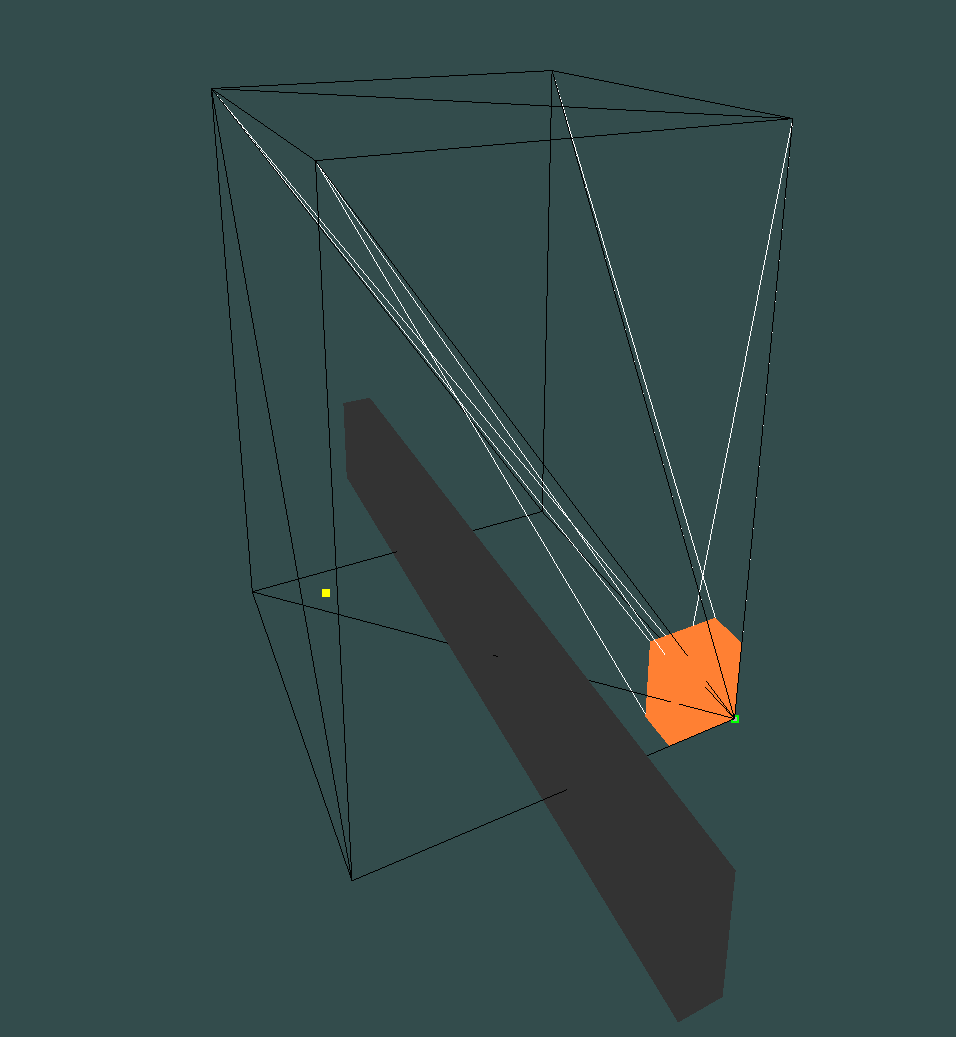
\includegraphics[height=0.6\textwidth]{kinematic_scaling_base_problem}
		\end{minipage}
		\begin{minipage}{0.5\textwidth}
			\centering
			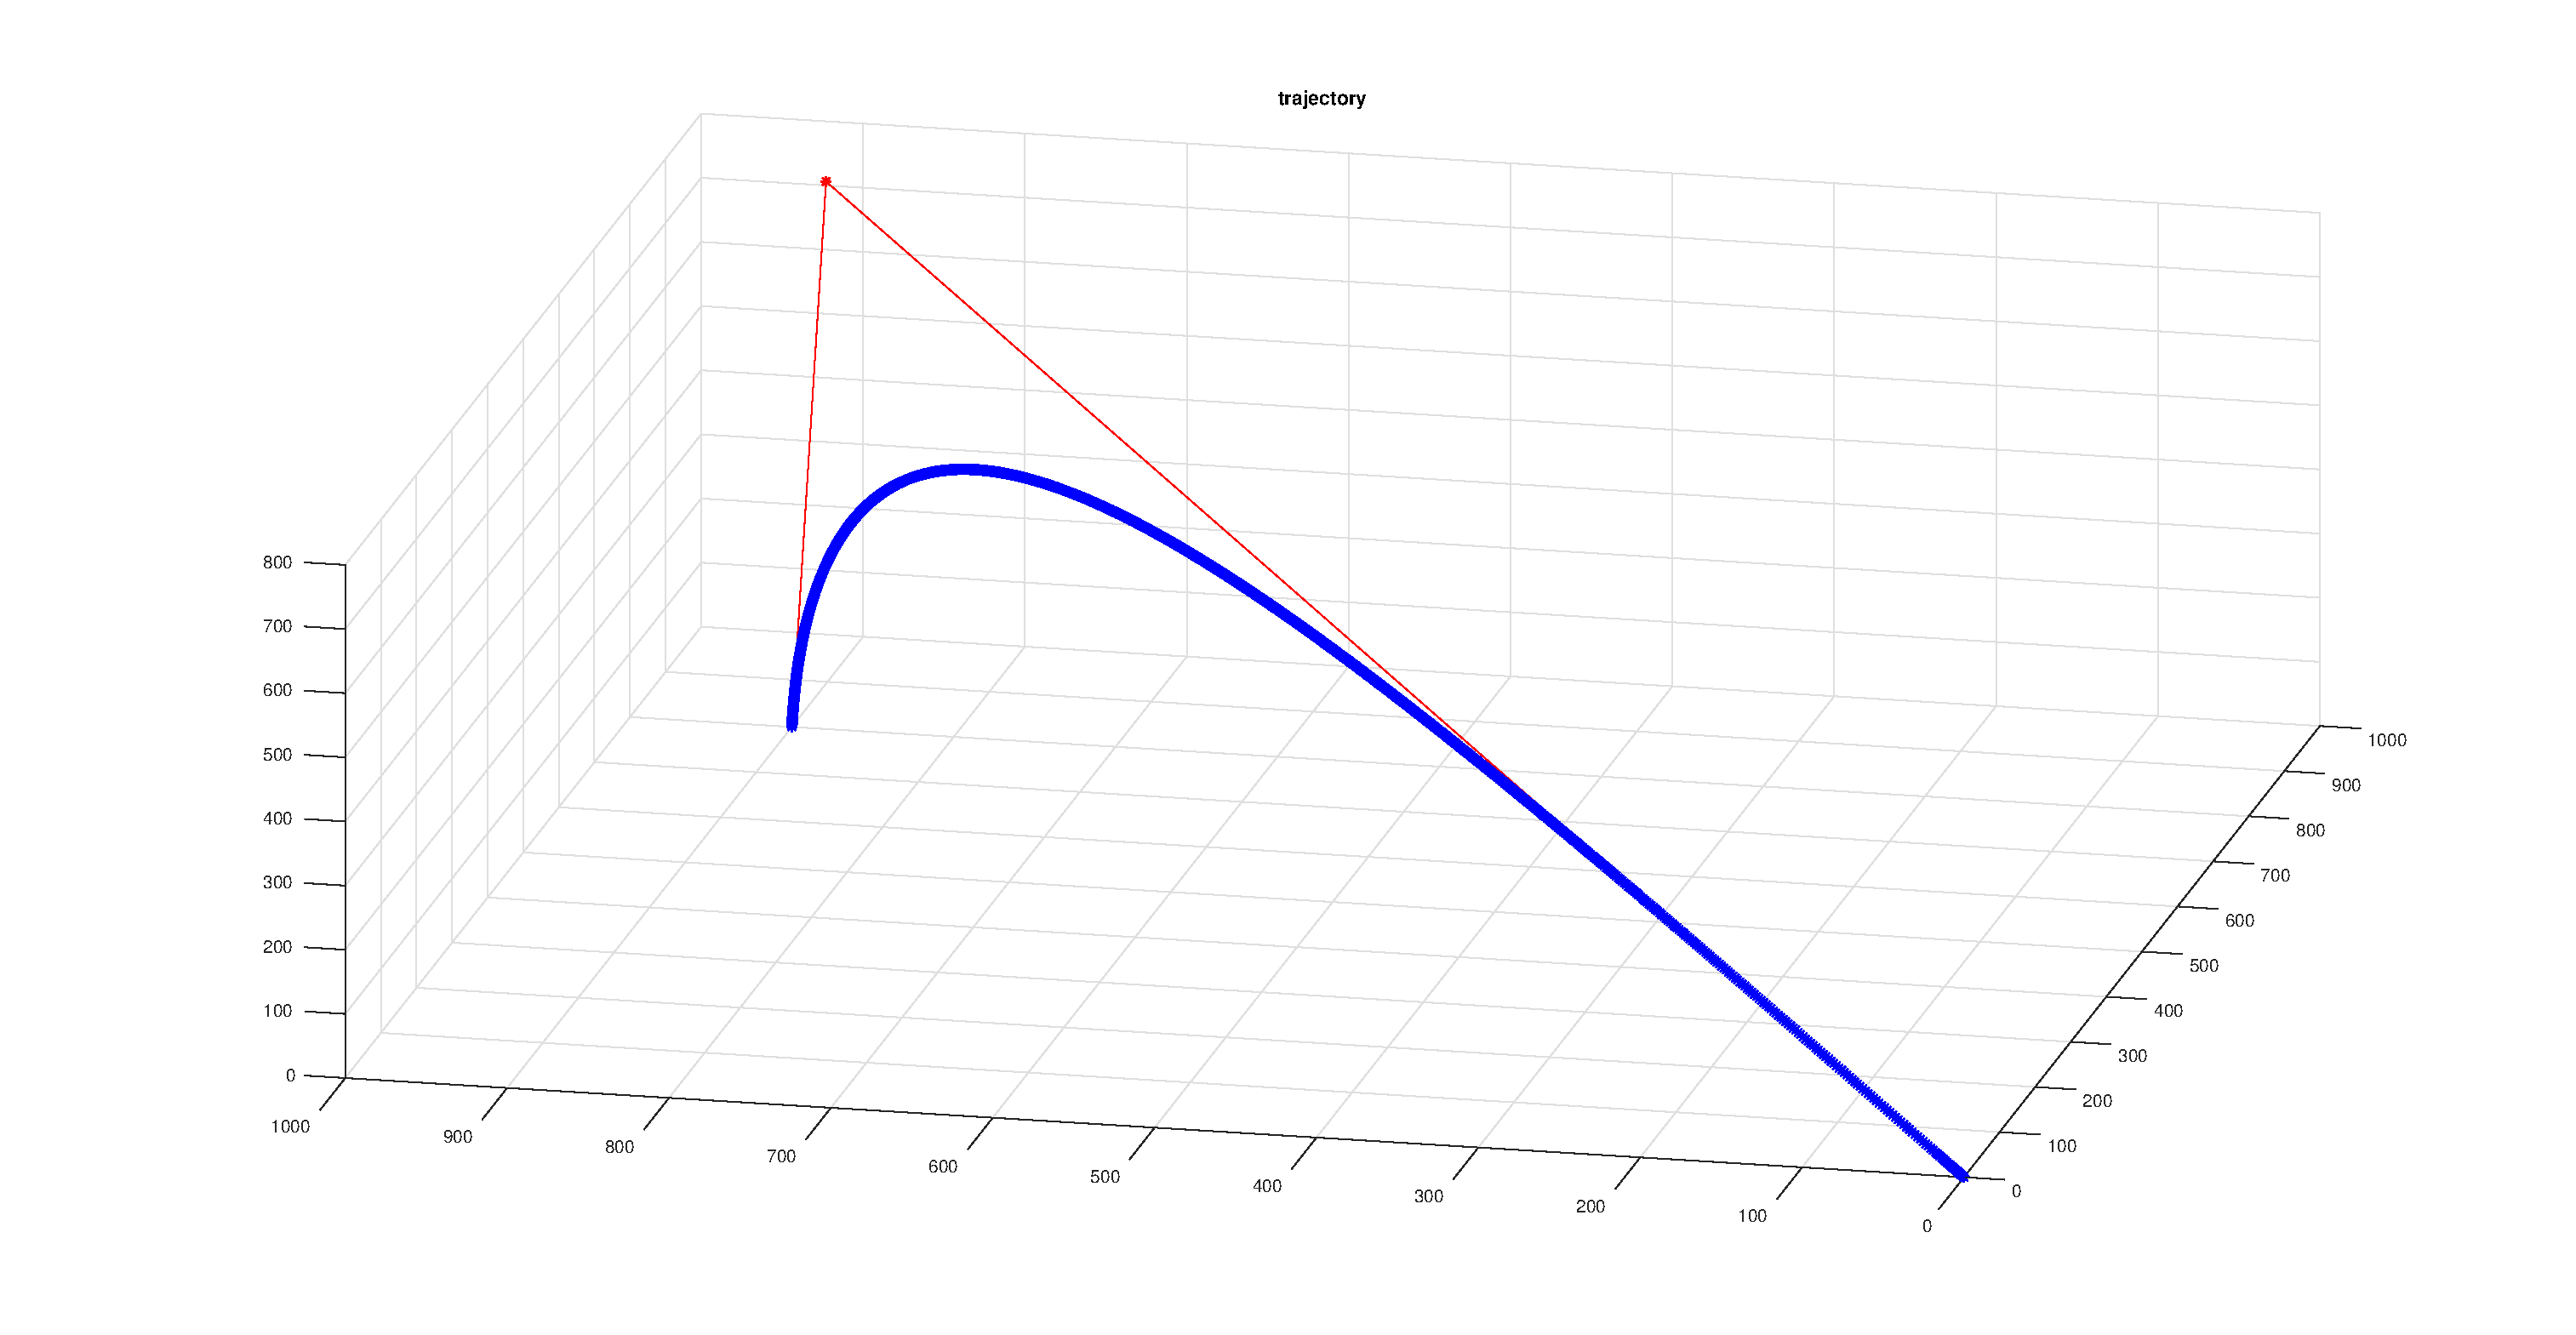
\includegraphics[height=0.6\textwidth]{motion_law_sample_problem_traj}
		\end{minipage}
		\caption[Motion Law Sample Problem]{Motion Law Sample Problem,
		left: problem layout, right: trajectory found}
		\label{fig:motion_law_sample_problem}
	\end{figure}

	\begin{figure}[hbt!]
		\centering
		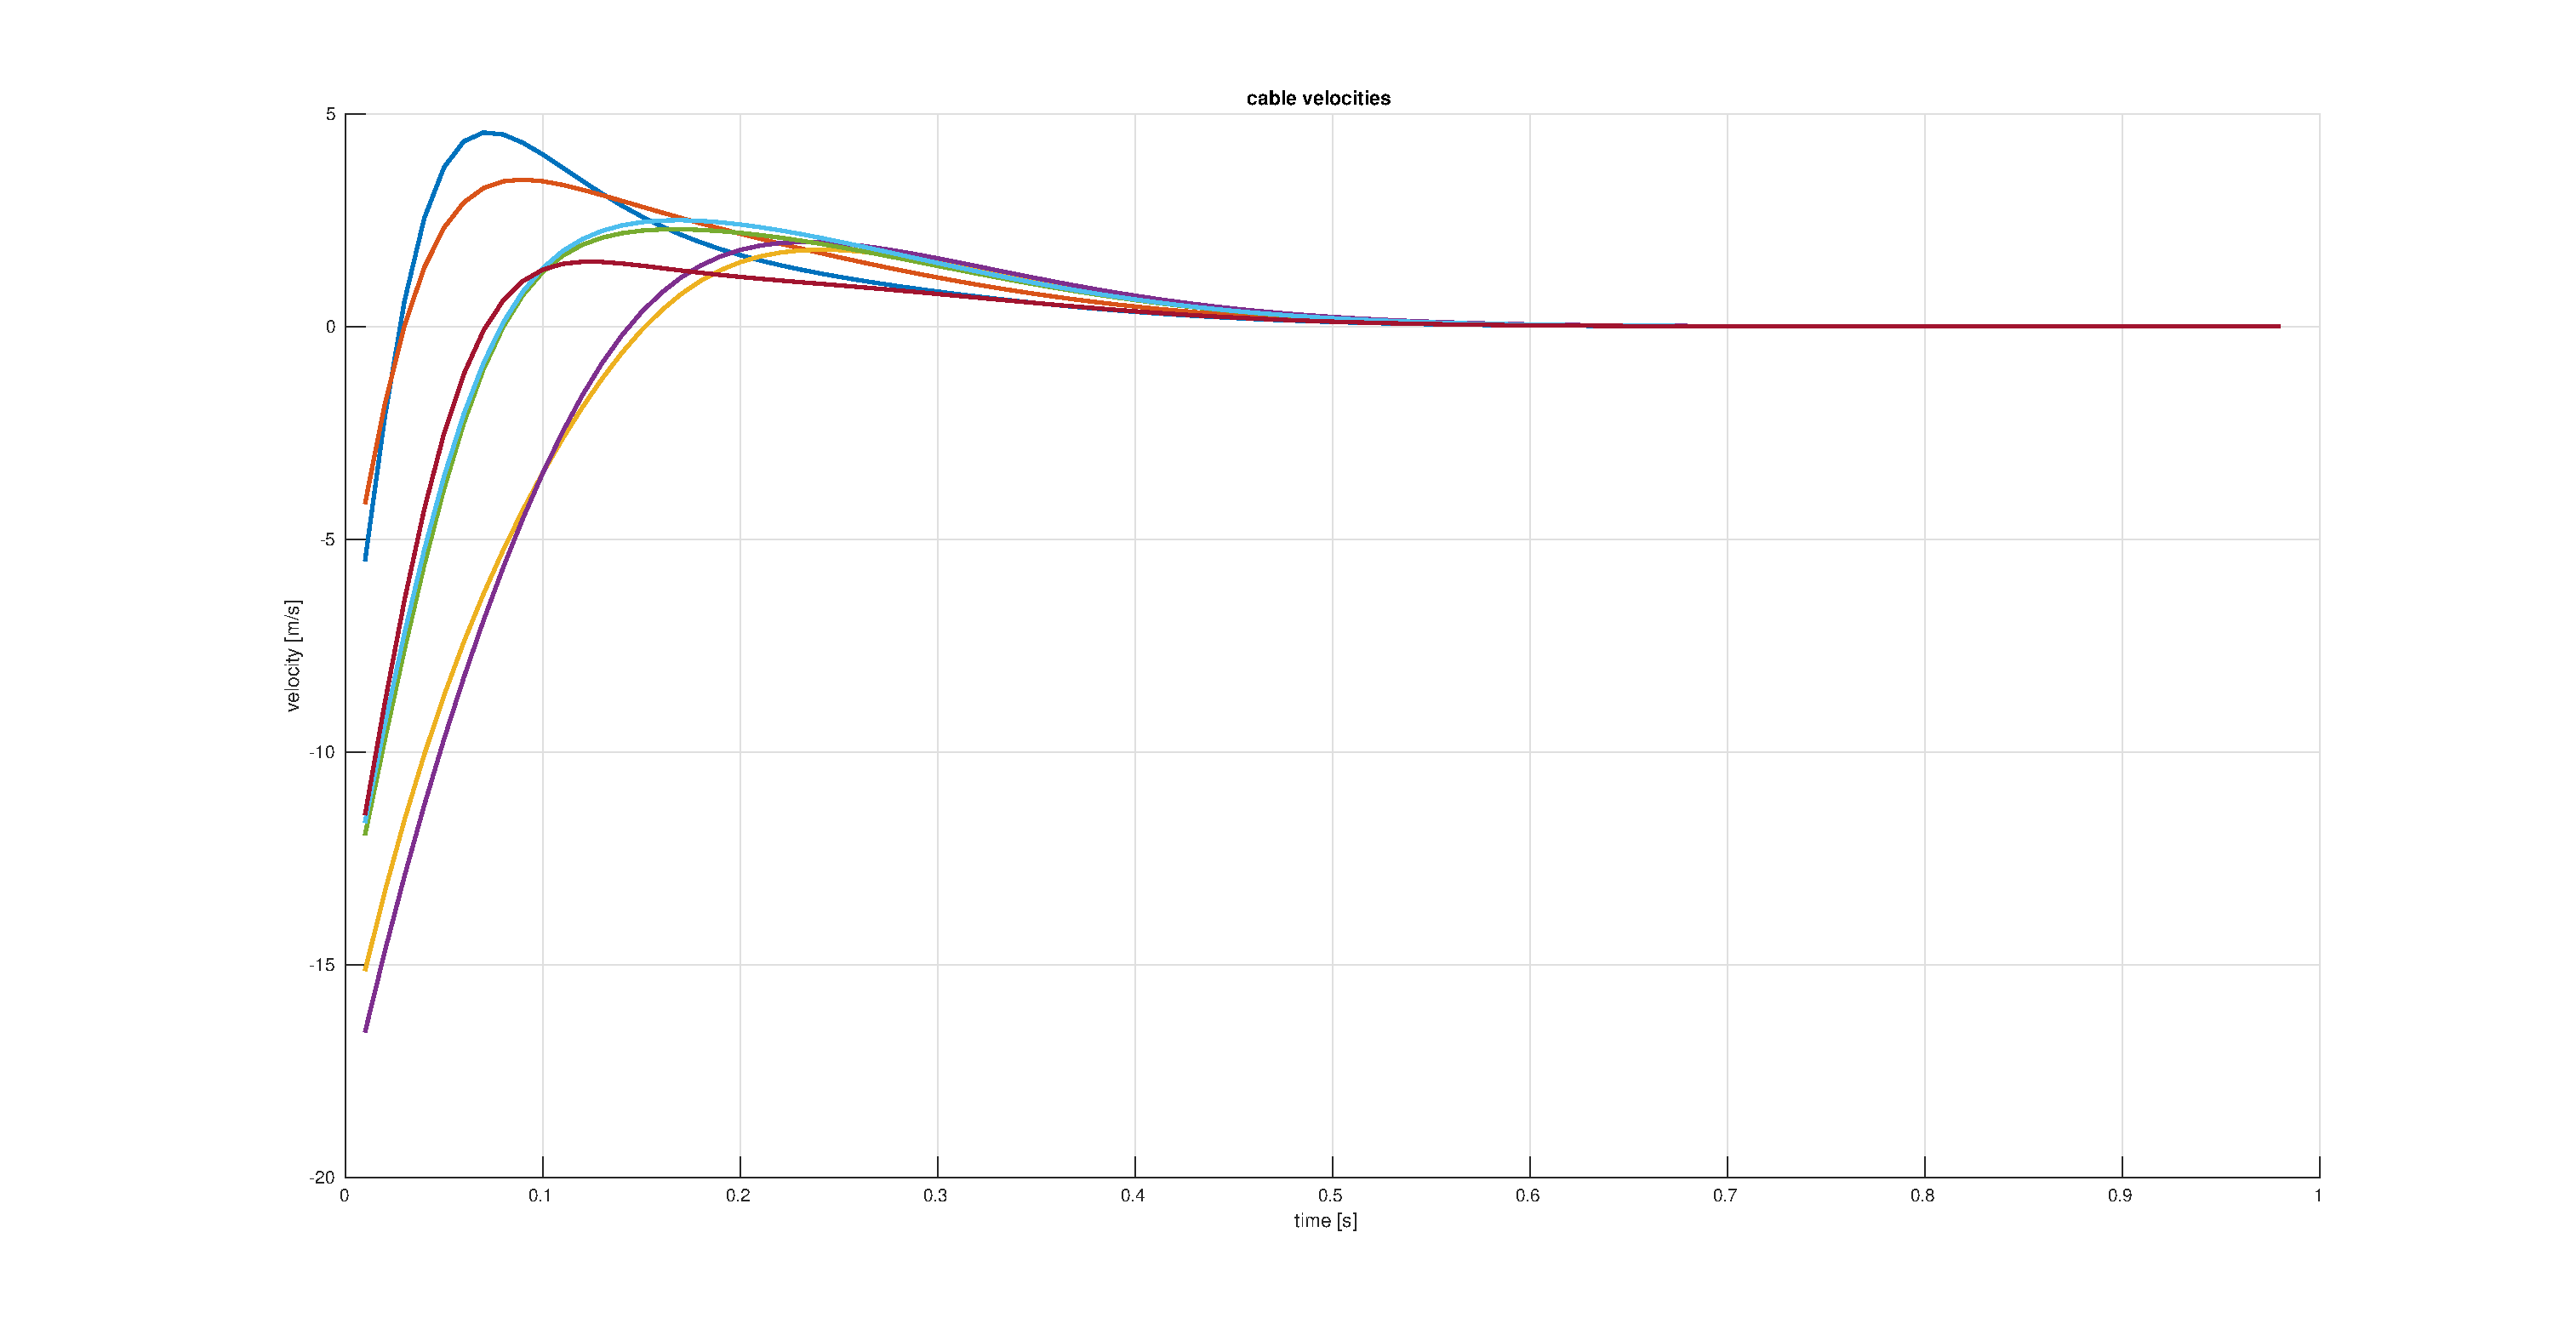
\includegraphics[width=\textwidth]{motion_law_base_velocities}
		\caption{Cable Velocities without Motion Law Scaling}
		\label{fig:cable_velocities_without_motion_law_scaling}
	\end{figure}

	\begin{figure}[hbt!]
		\centering
		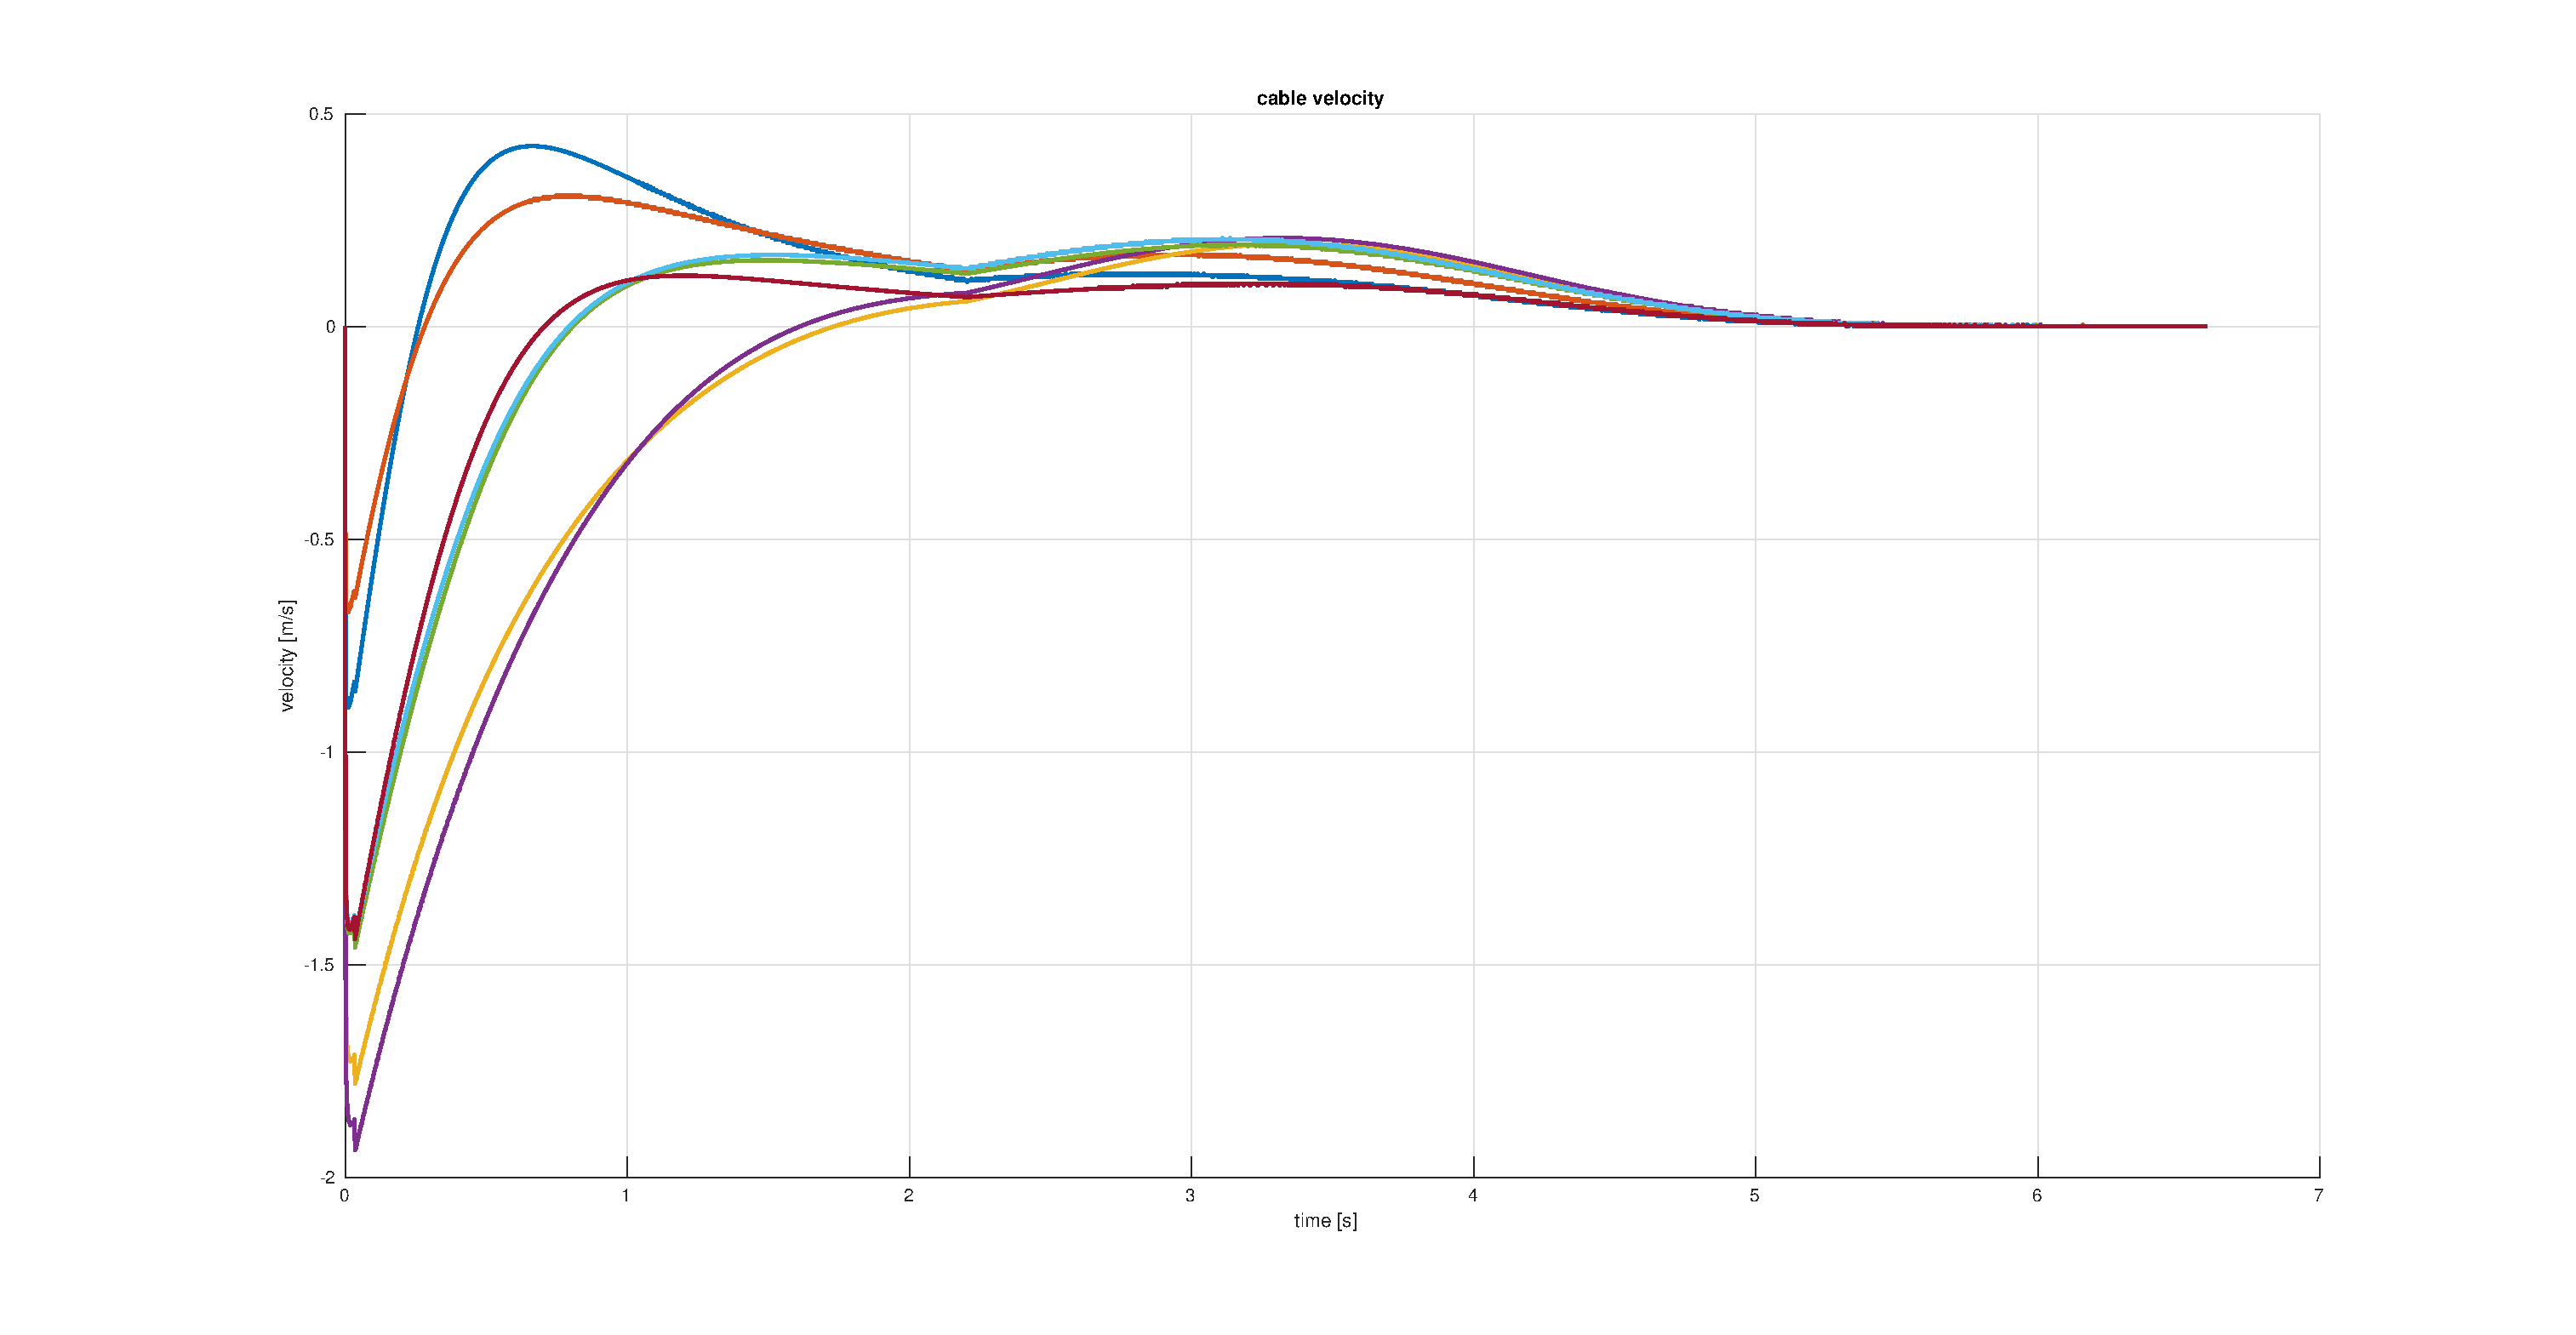
\includegraphics[width=\textwidth]{motion_law_output_velocities}
		\caption{Cable Velocities with Motion Law Scaling}
		\label{fig:cable_velocities_with_motion_law_scaling}
	\end{figure}

	\begin{figure}[hbt!]
		\centering
		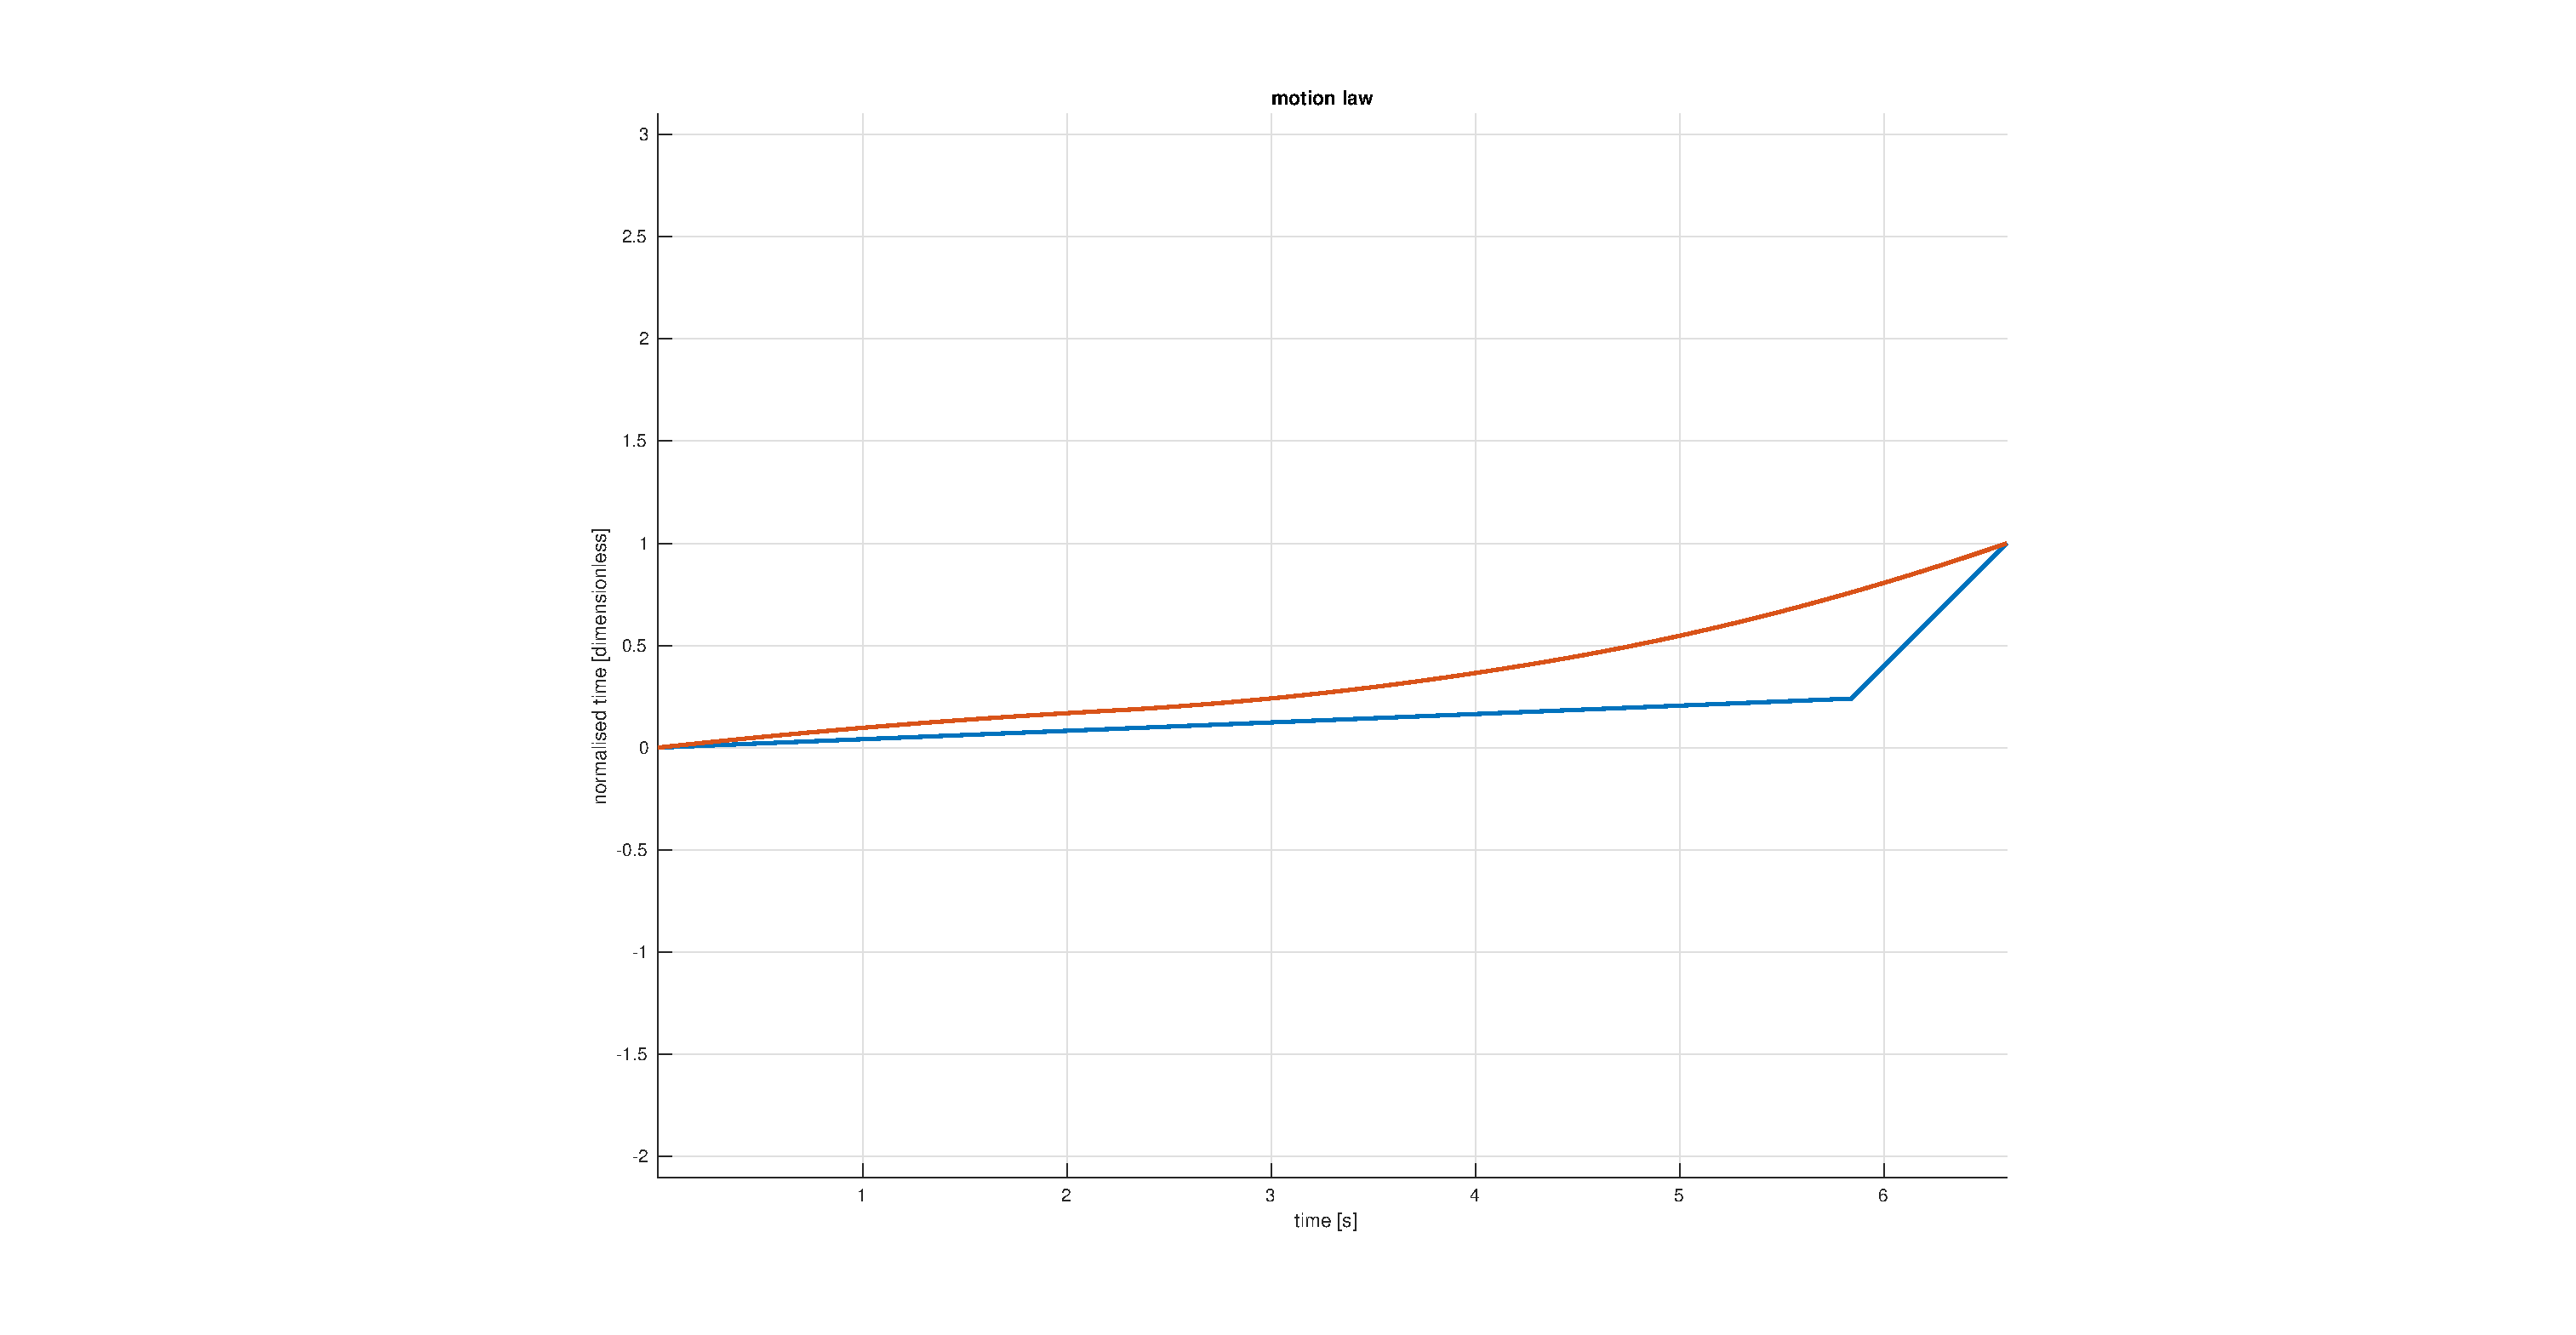
\includegraphics[width=\textwidth]{motion_law}
		\caption{Cable Velocities with Motion Law Scaling}
		\label{fig:motion_law}
	\end{figure}

	The output of the algorithm for this problem is shown in
	Figures~\ref{fig:cable_velocities_without_motion_law_scaling},
	\ref{fig:cable_velocities_with_motion_law_scaling} and~\ref{fig:motion_law}.
	In these figures, the algorithm attempted to find a motion law such that the
	maximum velocity does not exceed $2\si{\meter\per\second}$. For comparison,
	Figure~\ref{fig:cable_velocities_without_motion_law_scaling} shows the case
	where the algorithm is not applied ($\timesym \defeq \timenorm$). As can be
	seen, cable velocities reached up to $15\si{\meter\per\second}$ in this
	case. The motion law generated by the algorithm is reported in
	Figure~\ref{fig:motion_law}. In this figure both the control polygon and the
	B-Spline curve are shown. The output velocities found by applying this
	motion law is shown in
	Figure~\ref{fig:cable_velocities_with_motion_law_scaling}. As can be seen
	from the figurek the motion law succeeds in keeping the cables within their
	velocity bounds.

